\begin{figure}[h]
    \centering
    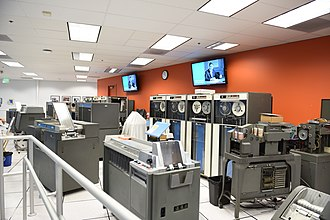
\includegraphics[scale=0.6]{IBM1401LABSETUP}
    \caption{Mainframe IBM 1401}
    \label{fig:IBM1401LABSETUP}
\end{figure}

Generasi ini ditandai dengan digunakannya transistor di dalam rangkaian sistem.
Transistor, yang diciptakan pada 1948 transistor oleh John Bardeen,
Walter Brattain, dan William Shockley, ketiganya merupakan
peneliti di Bell Labs di kala itu.

Teknologi transistor menggantikan tabung vakum yang ada di generasi kesatu. Trasistor
selain lebih kecil dibandingkan tabung vakum, jauh lebih hemat dalam penggunakan listrik,
hingga memungkinkan design sistem yang jauh lebih rumit dan juga lebih ``pintar``.

Selain digunakannya transistor, di generasi ini juga timbul teknologi \textit{Magnetic Core Memory}.
Teknologi ini jauh lebih efektif dan efisien dibandingkan teknologi penyimpanan sebelumnya.
\newpage
Salah satu contoh sistem komputer yang jatuh di generasi ini adalah IBM 1401 (lihat Gambar.\ref{fig:IBM1401LABSETUP}), komputer yang pada kala nya
sangat terkenal dan berhasil secara komersil.

\begin{figure}[h]
    \centering
    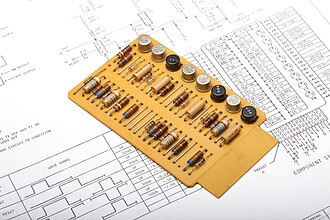
\includegraphics[scale=0.5]{IBM1401SMSCARD}
    \caption{Kartu Sirtkuit Transistor}
    \label{fig:IBM1401SMSCARD}
\end{figure}

Dengan menggunakan transistor, IBM 1401 memiliki arsitektur yang pada dasarnya adalah sekumpulan dioda-dioda
yang membentuk \textit{logic gate}, dan logic gate tersebut dimuat kedalam sebuah kartu seperti di Gambar.\ref{fig:IBM1401SMSCARD}

\begin{figure}[h]
    \centering
    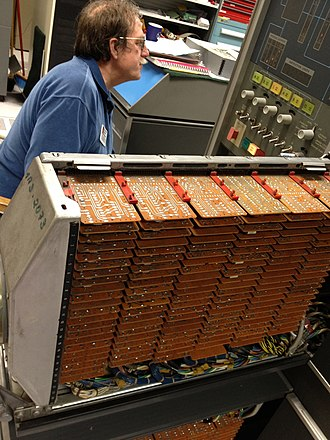
\includegraphics[scale=0.5]{IBM1401TRANSISTORS}
    \caption{Sirkuit Kartu Transistor}
    \label{fig:IBM1401TRANSISTORS}
\end{figure}

Dan kartu-kartu tersebut, atau SMS Card (\textit{Standard Modular System}) akan disusun menjadi sirkuit seperti di Gambar \ref{fig:IBM1401TRANSISTORS}.

Perkembangan atau tren yang timbul di generasi ini akan berlanjut ke generasi selanjutnya, terutama dalam hal mengecilnya ukuran komponen.
